\documentclass{article}
\usepackage{graphicx} % Required for inserting images
\usepackage{geometry}
 \geometry{
 a4paper,
 total={170mm,257mm},
 left=20mm,
 top=20mm,
 }
\title{Project Plan}
\author{ADAM JOHNSTONE - GLJD44}
\date{October 2024}

\begin{document}
\maketitle
\section{Project Plan}
Student name – Adam Johnstone\\
Supervisor name – Karl Southern\\
Project Title – Cryptanalysis of Retro Block Ciphers
\subsection{Project Description}
The modern world of cryptography is a fast-changing landscape with new and cutting-edge technology being developed year on year. Despite the ever-growing subject area, many older or retro techniques are still in use today. Throughout this project, I will be looking at retro block ciphers that can be considered predecessors to modern ciphers that are still in use today. Although some of the ciphers I will be looking at can be considered broken, it is a common practice in this field to test new attacks on older ciphers first to prove that they work before applying them to modern methods. To be more specific within this project I will mainly be talking about two retro block ciphers namely KASUMI and GOST.
First proposed in 2010 by  Dunkelman et al. \cite{C:DunKelSha10} the Sandwich Attack is a relatively new method of differential cryptanalysis that builds upon existing work concerning Related Key Boomerang (RKB) Attacks. In \cite{C:DunKelSha10} the sandwich attack is applied to the first seven rounds of the KASUMI cipher and achieves surprisingly good results which I will try to replicate in this project. Despite the results it appeared to have achieved the Sandwich Attack has not been utilised extensively with the only implementation I could find being by Jana et al.\cite{DBLP:journals/iacr/JanaRSP23} Due to its lack of implementation, I have decided to test the effectiveness of the Sandwich Attack on GOST as the main aim of this project. To define it better, I will be trying to answer the research question: Is the Sandwich Attack a feasible method for breaking the GOST block cipher?
\subsection{List of Deliverables}
Below is a list of deliverables split into three categories, with the basic deliverables being ones that I should achieve and are to be expected and advanced being ones that I would like to achieve but might not be feasible given external factors.
\subsubsection{Basic}
\maketitle {\large \textbf{Replication of the Sandwich attack on KASUMI}} \\
As the first part of my project, I will be replicating the implementation of the Sandwich Attack on KASUMI from the paper \cite{C:DunKelSha10}. This should allow me to gain a good understanding of how the Sandwich Attack works and whether its results are replicable.\\\\
\maketitle {\large \textbf{Replication of a Related Key Boomerang attack on GOST}}\\
Before I move on to doing a Sandwich attack on GOST I will first replicate an RKB Attack on GOST from \cite{DBLP:journals/iacr/Rudskoy10}. This will be used as a stepping stone stage as the Sandwich Attack builds upon RKB attacks and so I believe it will be useful to first understand RKB attacks before moving on to the Sandwich Attack.
\subsubsection{Intermediate}
\maketitle {\large \textbf{Establish the feasibility of the Sandwich Atack on GOST}}\\
Due to the Sandwich Attack having not yet been performed on the GOST block cipher, I think that it is first necessary to work through the mathematics of the cipher and the attack to work out the potential complexities (time and memory) of an implementation of the Sandwich Attack on GOST. The results from this stage of the project may lead to two different outcomes which I speak more about below.
\subsubsection{Advanced}
\maketitle {\large \textbf{Implement a Sandwich attack on GOST}}\\
Assuming that the previous stage of the project provides results that make an implementation of the Sandwich Attack on GOST feasible then the final stage of the project will be to do as such. Alongside the implementation, I will also try to prove my results from the previous stage with the practical implementation.\\\\
\maketitle {\large \textbf{Add to Sandwich attack documentation}}\\
Assuming that the previous stage of the project provides results that show an implementation of the Sandwich Attack on GOST is infeasible (complexity similar to brute force) then there is no point trying to implement the attack. Instead, I will then look to add to the documentation of the Sandwich Attack by providing worked examples and simpler explanations of its workings as these don’t currently exist and I believe they would be useful to the wider cryptology community.  
\subsection{Gantt Chart}
The below Gantt chart details my expected timelines for the deliverables of this project alongside the other submissions expected throughout the year. The submissions in the top half of the chart detail their hand-in dates however the deliverables do not have a fixed ‘due date’ and instead are rough guidelines. 
Due to having a busy schedule within the first term of this academic year, I am expecting to potentially run over the proposed timelines for the first two deliverables (replication of Sandwich attack on KASUMI and replication of RKB on GOST). Hence for the majority of the second term, I have only allocated the intermediate deliverable to allow some run over if needed. The final two lines in the Gantt chart show the Advanced deliverables which as discussed above will not (necessarily) both be completed so I have allocated them the same time slot.



\begin{figure}[hbt!]
    \centering
    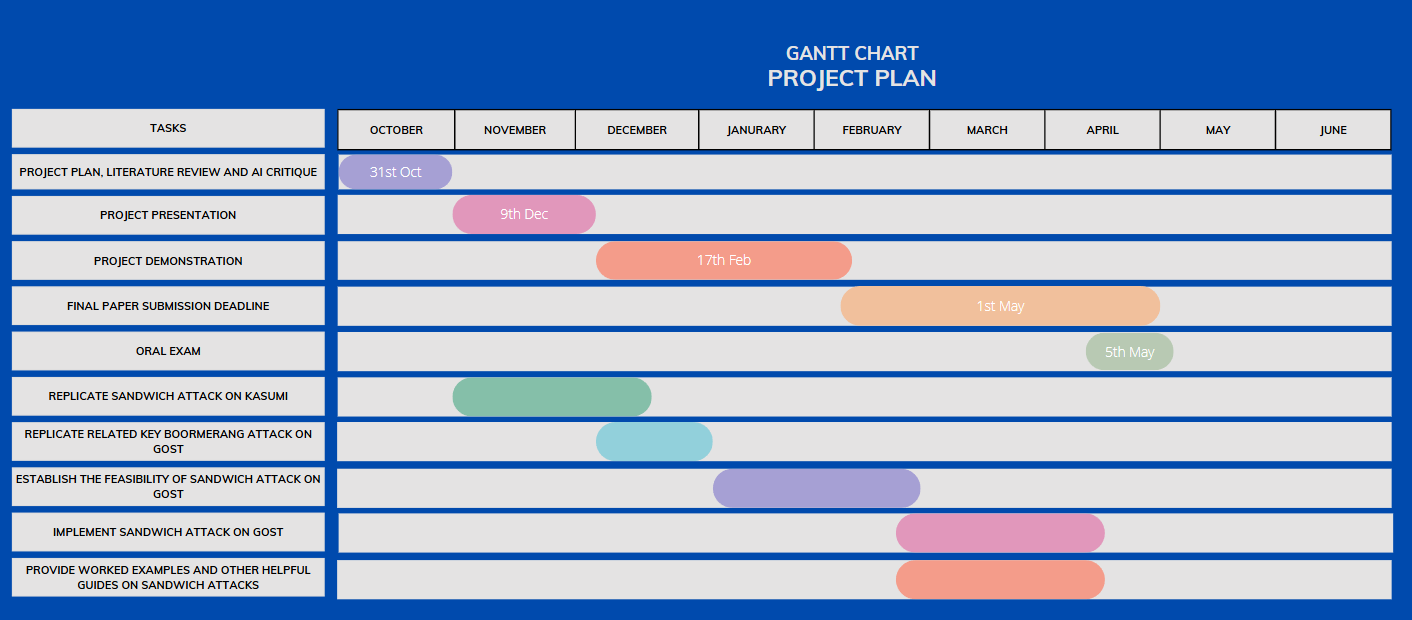
\includegraphics[width=1\linewidth]{ganttChart.png}
    \caption{Project Plan Gantt Chart}
    \label{fig:enter-label}
\end{figure}

\bibliographystyle{plain}
\bibliography{abbrev0,crypto, refs}



\end{document}
